\documentclass{article}

\usepackage{siunitx}
\usepackage[letterpaper]{geometry}
\usepackage{amsmath}
\usepackage{amssymb}
\usepackage{graphicx}

\def\scriptr{{\mbox{$\resizebox{.09in}{.08in}{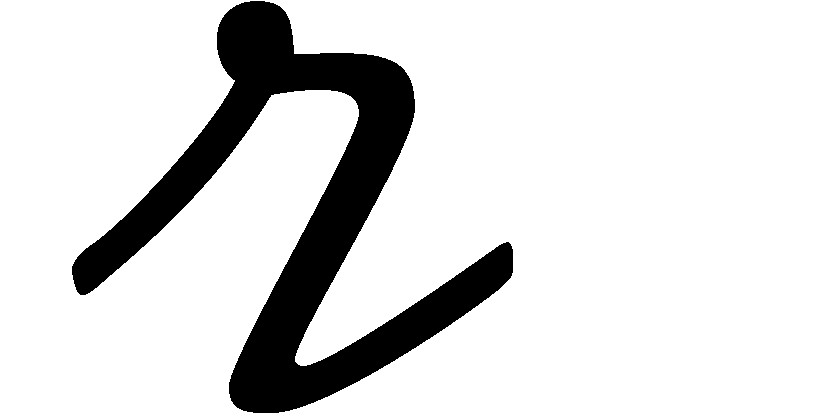
\includegraphics[trim= 1em 0 14em 0,clip]{ScriptR}}$}}}

\title{4132 HW 7}
\author{Duncan Wilkie}
\date{5 April 2022}

\begin{document}

\maketitle

\section*{1a}
Taking the Lorenz gauge,
\[\Box^{2}V=-\frac{1}{\epsilon_{0}}\rho \Rightarrow \rho=0\]
\[
  \Box^{2}\vec{A}--\mu_{0}\vec{J}
  \Rightarrow \nabla^{2}\left( \frac{1}{4\pi\epsilon_{0}}\frac{qt}{r^{2}}\hat{r} \right)-\mu_{0}\epsilon_{0}\frac{\partial^{2}}{\partial t^{2}}\left( \frac{1}{4\pi\epsilon_{0}}\frac{qt}{r^{2}} \right)\hat{r}=-\mu_{0}\vec{J}
\]
\[
  \Rightarrow \frac{1}{r^{2}}\frac{\partial}{\partial r}\left( r^{2}\frac{-1}{2\pi\epsilon_{0}}\frac{qt}{r^{3}}\hat{r} \right)
  -0 = -\mu_{0}\vec{J}
\]
\[
  \Rightarrow -\frac{qt}{2\pi\epsilon_{0}r^{2}}\frac{-1}{r^{2}}\hat{r}=-\mu_{0}\vec{J}
\]
\[
  \Rightarrow \vec{J}=-\frac{qt}{2\pi\epsilon_{0}\mu_{0}r^{4}}\hat{r}
\]

\section*{1b}
Under the given gauge,
\[
  V'=V-\frac{\partial \lambda}{\partial t}
  =\frac{1}{4\pi\epsilon_{0}}\frac{q}{r}
\]
and
\[
  \vec{A}'=\vec{A}+\nabla\lambda
  =\frac{1}{4\pi\epsilon_{0}}\frac{qt}{r^{2}}\hat{r}+\frac{1}{4\pi\epsilon_{0}}\frac{qt}{r^{2}}\hat{r}
  =\frac{1}{2\pi\epsilon_{0}}\frac{qt}{r^{2}}\hat{r}
\]
The first is simply the scalar potential due to a stationary point charge of magnitude $q$,
and the second is radially outward and therefore curl-free, resulting in a zero magnetic field,
also consistent with a stationary point charge.

\section*{2}
Applying the forced wave equation ansatz given in the text,
\[
  \vec{A}(\vec{r},t)=\frac{\mu_{0}}{4\pi}\int_{\mathbb{R}}\frac{J(\vec{r}',t)}{\scriptr}dV
\]
\[
  =\frac{\mu_{0}}{4\pi}\left( \int_{-b}^{-a}\frac{k\left( t-\frac{\scriptr}{c} \right)}{\scriptr}\hat{x}dx
    +\int_{a}^{b}\frac{k\left( t-\frac{\scriptr}{c}\right)}{\scriptr}\hat{x}dx
    +a\int_{0}^{\pi}\frac{k(t-\frac{\scriptr}{c})}{\scriptr}(-\hat{\theta})d\theta
    +b\int_{0}^{\pi}\frac{k(t-\frac{\scriptr}{c})}{\scriptr}(\hat{\theta})d\theta\right)
\]
The $x$ and $\theta$ dependence of $\scriptr$ is, since the potential is being calculated at the origin, $\scriptr=x/\cos\theta$.
Therefore,
\[
  =\frac{\mu_{0}}{4\pi}\bigg( \int_{-b}^{-a}\frac{k\cos\theta(t-\frac{cx}{\cos\theta})}{x}\hat{x}dx
    +\int_{a}^{b}\frac{k\cos\theta(t-\frac{cx}{\cos\theta})}{x}\hat{x}dx
    +a\int_{0}^{\pi}\frac{k(t-\frac{a}{c})}{a}(-\hat{\theta})d\theta
\]
\[
    +b\int_{0}^{\pi}\frac{k(t-\frac{b}{c})}{b}\hat{\theta}d\theta\bigg)
\]
\[
  =\frac{\mu_{0}}{4\pi}\left( \int_{-b}^{-a}\left( \frac{-kt}{x}-{ck}\right)\hat{x}dx
    +\int_{a}^{b}\left( \frac{kt}{x}-{ck} \right)\hat{x}dx
    +a\int_{0}^{\pi}\frac{k(t-\frac{a}{c})}{a}(-\hat{\theta})d\theta
    +b\int_{0}^{\pi}\frac{k(t-\frac{b}{c})}{b}\hat{\theta}d\theta\right)
\]
\[
  \frac{\mu_{0}}{4\pi}\left( -kt\ln(x)\bigg|_{-b}^{-a}\hat{x}-ckx\bigg|_{-a}^{-b}\hat{x}
    +kt\ln(x)\bigg|_{a}^{b}\hat{x}-ckx\bigg|_{a}^{b}\hat{x}
    -kt\pi\hat{\theta}+\frac{ak}{c}\pi\hat{\theta}
    +kt\pi\hat{\theta}-\frac{bk}{c}\pi\hat{\theta}\right)
\]
\[
  \frac{\mu_{0}}{4\pi}\left( 2kt\ln\frac{b}{a}\hat{x}+\pi \frac{k}{c}\left[ a-b \right]\hat{\theta}\right)
\]
Its derivative with respect to time is nonzero at
\[\frac{\partial\vec{A}}{\partial t}=\frac{\mu_{0}k}{2\pi}\ln\frac{b}{a}\hat{x}\]
Since the potential and therefore its gradient is zero, the electric field is the negative of the above.
The magnetic field is incalculable because the curl of $\vec{A}$ cannot be determined from a single point.

\section*{3}
The scalar potential is
\[V(\vec{r},t)=\frac{1}{4\pi\epsilon_{0}}\frac{qc}{|\scriptr| c-\scriptr\cdot v}\]
The position of the charge at time $t$ is, in cylindrical coordinates, $r'=a\hat{r}+\omega t\hat{\theta}$.
We may then write
\[\scriptr = {r}-r'=(r-a)\hat{r}+(\theta-\omega t)\hat{\theta}+z\hat{z}\]
The velocity of the charge in cylindrical coordinates is
\[v=\dot{r}\hat{r}+r\dot{\theta}\hat{\theta}+\dot{z}\hat{z}=a\omega\hat{\theta}\]
Plugging this in to the scalar potential,
\[
  V(r,\theta,z,t)=\frac{1}{4\pi\epsilon_{0}}\frac{qc}{a\omega(\omega t-\theta)+c\sqrt{(r-a)^{2}+(\theta-\omega t)^{2}+z^{2}}}
\]
On the $z$-axis, $r=\theta=0$, so
\[V(z,t)=\frac{1}{4\pi\epsilon_{0}}\frac{qc}{at\omega^{2}-c\sqrt{a^{2}+\omega^{2}t^{2}+z^{2}}}\]
The vector potential is
\[
  \vec{A}(\vec{r},t)=\frac{v}{c^{2}}V(\vec{r},t)
  =\frac{a\omega\hat{\theta}}{c^{2}}\frac{1}{4\pi\epsilon_{0}}\frac{qc}{a\omega(\omega t-\theta)
    +c\sqrt{(r-a)^{2}+(\theta-\omega t)^{2}+z^{2}}}
\]
On the $z$-axis, this becomes
\[\vec{A}(z,t)=\frac{1}{4\pi\epsilon_{0}c}\frac{a\omega q}{at\omega^{2}-c\sqrt{a^{2}+\omega^{2}t^{2}+z^{2}}}\hat{\theta}\]

\section*{4}
The expression for the electric field of a moving charge is, using the equation from the book,
\[
  \vec{E}=\frac{q}{4\pi\epsilon_{0}}\frac{\scriptr}{(\vec{\scriptr}\cdot\vec{u})^{3}}
  \left[ (c^{2}-v^{2})\vec{u}+\vec{\scriptr}\times(\vec{u}\times\vec{a}) \right]
\]
where $\vec{u}=c\hat{\scriptr}-\vec{v}$ and $\vec{a}$ is the acceleration of the particle.
In this case, the cross products are zero since everything's confined to a line, and the dot products are the scalar product of signed magnitudes, so
\[
  \vec{E}=\frac{q}{4\pi\epsilon_{0}}\frac{\scriptr}{[\scriptr(c-v)]^{3}}(c^{2}-v^{2})(c-v)\hat{x}
  =\frac{q}{4\pi\epsilon_{0}}\frac{1}{\scriptr^{2}}\frac{c^{2}-v^{2}}{(c-v)^{2}}\hat{x}
  =\frac{q}{4\pi\epsilon_{0}}\frac{1}{\scriptr^{2}}\frac{(c+v)(c-v)}{(c-v)^{2}}\hat{x}
  =\frac{q}{4\pi\epsilon_{0}}\frac{1}{\scriptr^{2}}\frac{c+v}{c-v}\hat{x}
\]
This is the given expression, save for the factor of $q$ missing in the assignment which I presume is a copying error.
The magnetic field is, using the equation given in the same chapter,
\[
  \vec{B}=\frac{1}{c}\hat{\scriptr}\times\vec{E}
\]
This cross product is zero, since $\hat{\scriptr}=\hat{x}$ and $\vec{E}$ was found to lie along the $x$-axis.

\section*{5a}
For a point distance $d$ from the wire, the distance from a differential charge element $dq=\lambda Rd\theta$ may be written in terms of angle as
$R=d/\sin(\theta)$, as the distance from the wire forms a right triangle with opposite $d$ and hypotenuse $R$.
Substituting this result and integrating over all $dq$,
\[
  \vec{E}=\int_{0}^{\pi}\frac{\lambda Rd\theta}{4\pi\epsilon_{0}}\frac{1-v^{2}/c^{2}}{(1-v^{2}\sin^{2}\theta/c^{2})^{3/2}}\frac{\hat{R}}{R^{2}}
  =\frac{\lambda(1-v^{2}/c^{2})}{4\pi\epsilon_{0}}\overline{\hat{R}}
  \int_{0}^{\pi}\frac{1}{(1-v^{2}\sin^{2}\theta/c^{2})^{3/2}}\frac{1}{d/\sin\theta}d\theta
\]
\[
  =\frac{\lambda(1-v^{2}/c^{2})}{4\pi\epsilon_{0}d}\overline{\hat{R}}\int_{0}^{\pi}\frac{\sin\theta}{(1-v^{2}\sin^{2}\theta/c^{2})^{3/2}}d\theta
\]
Sympy says the nasty integral evaluates to $\frac{2}{1-v^{2}/c^{2}}$, so the electric field is
\[\vec{E}=\frac{\lambda}{2\pi\epsilon_{0}d}\hat{r}\]
\section*{5b}
The magnetic field is, in the constant-velocity case,
\[
  \vec{B}=\frac{1}{c^{2}}(\vec{v}\times\vec{E})
  =\frac{\lambda v}{2\pi\epsilon_{0}c^{2}d}\hat{\theta}=\frac{\mu_{0}I}{2\pi d}\hat{\theta}
\]
where the velocity is taken in the $\hat{z}$ direction and we have used $c^{2}=\frac{1}{\mu_{0}\epsilon_{0}}$.
Both of these agree with the easy derivations from Coulomb's and Ampere's laws.




\end{document}

%%% Local Variables:
%%% mode: latex
%%% TeX-master: t
%%% End:
